\chapter*{APPENDICES}
\addcontentsline{toc}{chapter}{APPENDICES}
{\baselineskip=1\baselineskip

	
\includepdf[
		pages=1,
		scale=0.9,
		pagecommand={
				\chapter*{APPENDIX A \\ \normalfont LETTER OF CONSENT}
				\addcontentsline{toc}{chapter}{APPENDIX B}
				\vspace{1cm}
			},
		offset=0 -3cm
	]{appendix_pdf/appendix_b.pdf}

	
\includepdf[pages=2-, pagecommand={}, scale=0.9]{appendix_pdf/appendix_b.pdf}

	\chapter*{APPENDIX B \\ \normalfont INTERVIEW CONDUCTED}
	\addcontentsline{toc}{chapter}{APPENDIX B}

	\begin{longtable}{|p{4cm}|p{10cm}|}
		\hline
		\textbf{Interviewer(s)} & Jason T. Daohog / Jeushian Ritz Reblando / Novem Kate Barbosa                                                                                                \\ \hline
		\textbf{Note Taker}     & John Patrick Rautraut                                                                                                                                        \\ \hline
		\textbf{Observer}       & Joel F. Sabuero Jr.                                                                                                                                          \\ \hline
		\textbf{Location}       & Janog Cacao Plantation, Initao, Misamis Oriental                                                                                                             \\ \hline
		\multicolumn{2}{|l|}{\textbf{Date:} 10-5-2025 \hspace{1cm} \textbf{Start Time:} 1:30 PM \hspace{1cm} \textbf{End Time:} 4:00 PM}                                                       \\ \hline
		\textbf{Objectives}     & To understand existing farming practices, identify challenges in disease detection and management, and collect essential information for system development. \\ \hline

		\multicolumn{2}{|l|}{\textbf{Name (Ngalan) (optional): \underline{Erlinda Janog}
		}}                                                                                                                                                                                     \\
		\multicolumn{2}{|l|}{\textbf{Age (Edad):}}                                                                                                                                             \\

		\multicolumn{2}{|p{12cm}|}{\vspace{0.1cm} \textbf{1.} How big is your cacao farm?}                                                                                                     \\
		\multicolumn{2}{|p{12cm}|}{\textit{Pila kadako imong umahan sa kakaw? (sa hectares o square meters)}}                                                                                  \\
		\multicolumn{2}{|p{12cm}|}{\textbf{5 hectares}}                                                                                                                                        \\

		\multicolumn{2}{|p{12cm}|}{\vspace{0.1cm}  \textbf{2.} Does the size make your work harder or easier each day?}                                                                        \\
		\multicolumn{2}{|p{12cm}|}{\textit{Ang kadako ba sa imong uma makapadali o makalisod sa imong trabaho adlaw-adlaw?}}                                                                   \\
		\multicolumn{2}{|p{12cm}|}{\textbf{It makes the work harder since the area is large, and it takes more time to check all trees and manage spraying or pruning}}                        \\

		\multicolumn{2}{|p{12cm}|}{\vspace{0.1cm} \textbf{3.} How do you usually enter your farm when you check the trees? (by road, by foot, etc.)}                                           \\
		\multicolumn{2}{|p{12cm}|}{\textit{Giunsa nimo kasagaran pag-agi sa umahan kung mag-inspeksiyon ka sa mga kahoy?}}                                                                     \\
		\multicolumn{2}{|p{12cm}|}{\textbf{By foot}}                                                                                                                                           \\

		\multicolumn{2}{|p{12cm}|}{\vspace{0.1cm} \textbf{4.} What problems do you face when going around your farm?}                                                                          \\
		\multicolumn{2}{|p{12cm}|}{\textit{Unsa nga mga problema imong makita kung mubisita ka sa uma?}}                                                                                       \\
		\multicolumn{2}{|p{12cm}|}{\textbf{Spray, pruning, danggan, rain}}                                                                                                                     \\
		\multicolumn{2}{|p{12cm}|}{\vspace{0.1cm} \textbf{5.} Are there things like tall trees, hills, rivers, or power lines in or near your farm?}                                           \\
		\multicolumn{2}{|p{12cm}|}{\textit{Naa bay mga taas nga kahoy, bungtod, sapa, o mga kuryente nga linya sa sulod o duol sa umahan?}}                                                    \\
		\multicolumn{2}{|p{12cm}|}{\textbf{Yes}}                                                                                                                                               \\

		\multicolumn{2}{|p{12cm}|}{\vspace{0.1cm} \textbf{6.} How do these affect your work with the cacao trees?}                                                                             \\
		\multicolumn{2}{|p{12cm}|}{\textit{Pa-unsa ni siya naka-apekto sa imong pagtrabaho sa umahan?}}                                                                                        \\
		\multicolumn{2}{|p{12cm}|}{\textbf{No}}                                                                                                                                                \\

		\multicolumn{2}{|p{12cm}|}{\vspace{0.1cm} \textbf{7.} What is the first thing you see when a cacao pod is diseased? (color, spots, wilting, etc.)}                                     \\
		\multicolumn{2}{|p{12cm}|}{\textit{Unsay unang butang nga imong makita kung ang bunga sa kakaw kay naay daut? (kolor, naay mansa, ug uban pa)}}                                        \\
		\multicolumn{2}{|p{12cm}|}{\textbf{Appearance}}                                                                                                                                        \\

		\multicolumn{2}{|p{12cm}|}{\vspace{0.1cm} \textbf{8.} What signs do you look for before you say a cacao is unhealthy?}                                                                 \\
		\multicolumn{2}{|p{12cm}|}{\textit{Unsa ang mga timailhan nga imong tan-awon una kung ang kakaw kay daut?}}                                                                            \\
		\multicolumn{2}{|p{12cm}|}{\textbf{Color dots, phytophthora}}                                                                                                                          \\

		\multicolumn{2}{|p{12cm}|}{\vspace{0.1cm} \textbf{9.} How do you remember which tree has a diseased cacao? (notebook, marking, memory, etc.)}                                          \\
		\multicolumn{2}{|p{12cm}|}{\textit{Giunsa nimo paghinumdom kung asa nga mga kahoy ang naay daut nga kakaw? (notebook, marka, hinumdoman ra, ug uban pa)}}                              \\
		\multicolumn{2}{|p{12cm}|}{\textbf{The affected tree won’t affect another tree. It will only affect the pods in that affected tree}}                                                   \\

		\multicolumn{2}{|p{12cm}|}{\vspace{0.1cm} \textbf{10.} When you see a diseased cacao pod, what do you do first? (cut, spray, remove, etc.)}                                            \\
		\multicolumn{2}{|p{12cm}|}{\textit{Kung makakita kag bunga sa kakaw nga daut, unsa imong buhaton una? (putlon, sprayan, tangtangon, ug uban pa)}}                                      \\
		\multicolumn{2}{|p{12cm}|}{\textbf{Spray, unnoticed due to other}}                                                                                                                     \\

		\multicolumn{2}{|p{12cm}|}{\vspace{0.1cm} \textbf{11.} Which methods work best for you to control disease?}                                                                            \\
		\multicolumn{2}{|p{12cm}|}{\textit{Unsa ang mga pamaagi ang mas epektibo para nimo aron makontrol ang daut?}}                                                                          \\
		\multicolumn{2}{|p{12cm}|}{\textbf{Pest control spray}}                                                                                                                                \\

		\multicolumn{2}{|p{12cm}|}{\vspace{0.1cm} \textbf{12.} Which ones do not work well?}                                                                                                   \\
		\multicolumn{2}{|p{12cm}|}{\textit{Unsang mga pamaagi ang dili kaayo epektibo?}}                                                                                                       \\
		\multicolumn{2}{|p{12cm}|}{\textbf{Wrapping pods with plastic during the rainy season, since it causes mold formation.}}                                                               \\

		\multicolumn{2}{|p{12cm}|}{\vspace{0.1cm} \textbf{13.} How do you decide if you will treat, cut, or remove the sick pod?}                                                              \\
		\multicolumn{2}{|p{12cm}|}{\textit{Giunsa nimo pagpili kung tambalan, putlon, o tangtangon ang daut nga bunga?}}                                                                       \\
		\multicolumn{2}{|p{12cm}|}{\textbf{Remove only}}                                                                                                                                       \\

		\multicolumn{2}{|p{12cm}|}{\vspace{0.1cm} \textbf{14.} How many times do you check your cacao for disease? (per week or per month)}                                                    \\
		\multicolumn{2}{|p{12cm}|}{\textit{Kapila ka mag-inspeksiyon sa mga daut na kakaw? (kada semana o kada bulan)}}                                                                        \\
		\multicolumn{2}{|p{12cm}|}{\textbf{Everyday (3 weeks per area)}}                                                                                                                       \\

		\multicolumn{2}{|p{12cm}|}{\vspace{0.1cm} \textbf{15.} Do you check more often in the rainy or dry season?}                                                                            \\
		\multicolumn{2}{|p{12cm}|}{\textit{Mas kanunay ba ka mag-inspeksiyon sa ting-uwan o sa ting-init?}}                                                                                    \\
		\multicolumn{2}{|p{12cm}|}{\textbf{Both. Especially during rainy seasons, each pod should not be wrapped in a plastic since it will mold except for those who are already wrapped}}    \\

		\multicolumn{2}{|p{12cm}|}{\vspace{0.1cm} \textbf{16.} What problems do you face when checking your cacao for disease?}                                                                \\
		\multicolumn{2}{|p{12cm}|}{\textit{Unsa nga mga problema imong naagian kung mag-inspeksiyon ka sa mga daut nga kakaw?}}                                                                \\
		\multicolumn{2}{|p{12cm}|}{\textbf{Sometimes it’s hard to see the pods because of the rain and thick leaves.}}                                                                         \\

		\multicolumn{2}{|p{12cm}|}{\vspace{0.1cm} \textbf{17.} Can you tell a story when you found a disease too late?}                                                                        \\
		\multicolumn{2}{|p{12cm}|}{\textit{Pwede nimo mahulagway pag diskobre nimo nga ulahi na nakita nga daut ang kakaw?}}                                                                   \\
		\multicolumn{2}{|p{12cm}|}{\textbf{It happened during the rainy days when I couldn’t check the trees. When I came back, some of the pods were already black and rotten}}               \\

		\multicolumn{2}{|p{12cm}|}{\vspace{0.1cm} \textbf{18.} What happened to your harvest after that?}                                                                                      \\
		\multicolumn{2}{|p{12cm}|}{\textit{Unsay nahitabo sa imong ani pagkahuman ato?}}                                                                                                       \\
		\multicolumn{2}{|p{12cm}|}{\textbf{Harvest 5-7 kilo (Peak season duing november to december)}}                                                                                         \\ \hline

		\multicolumn{2}{|p{12cm}|}{%
		\textbf{Documentation: \vspace{0.4cm}} \par
		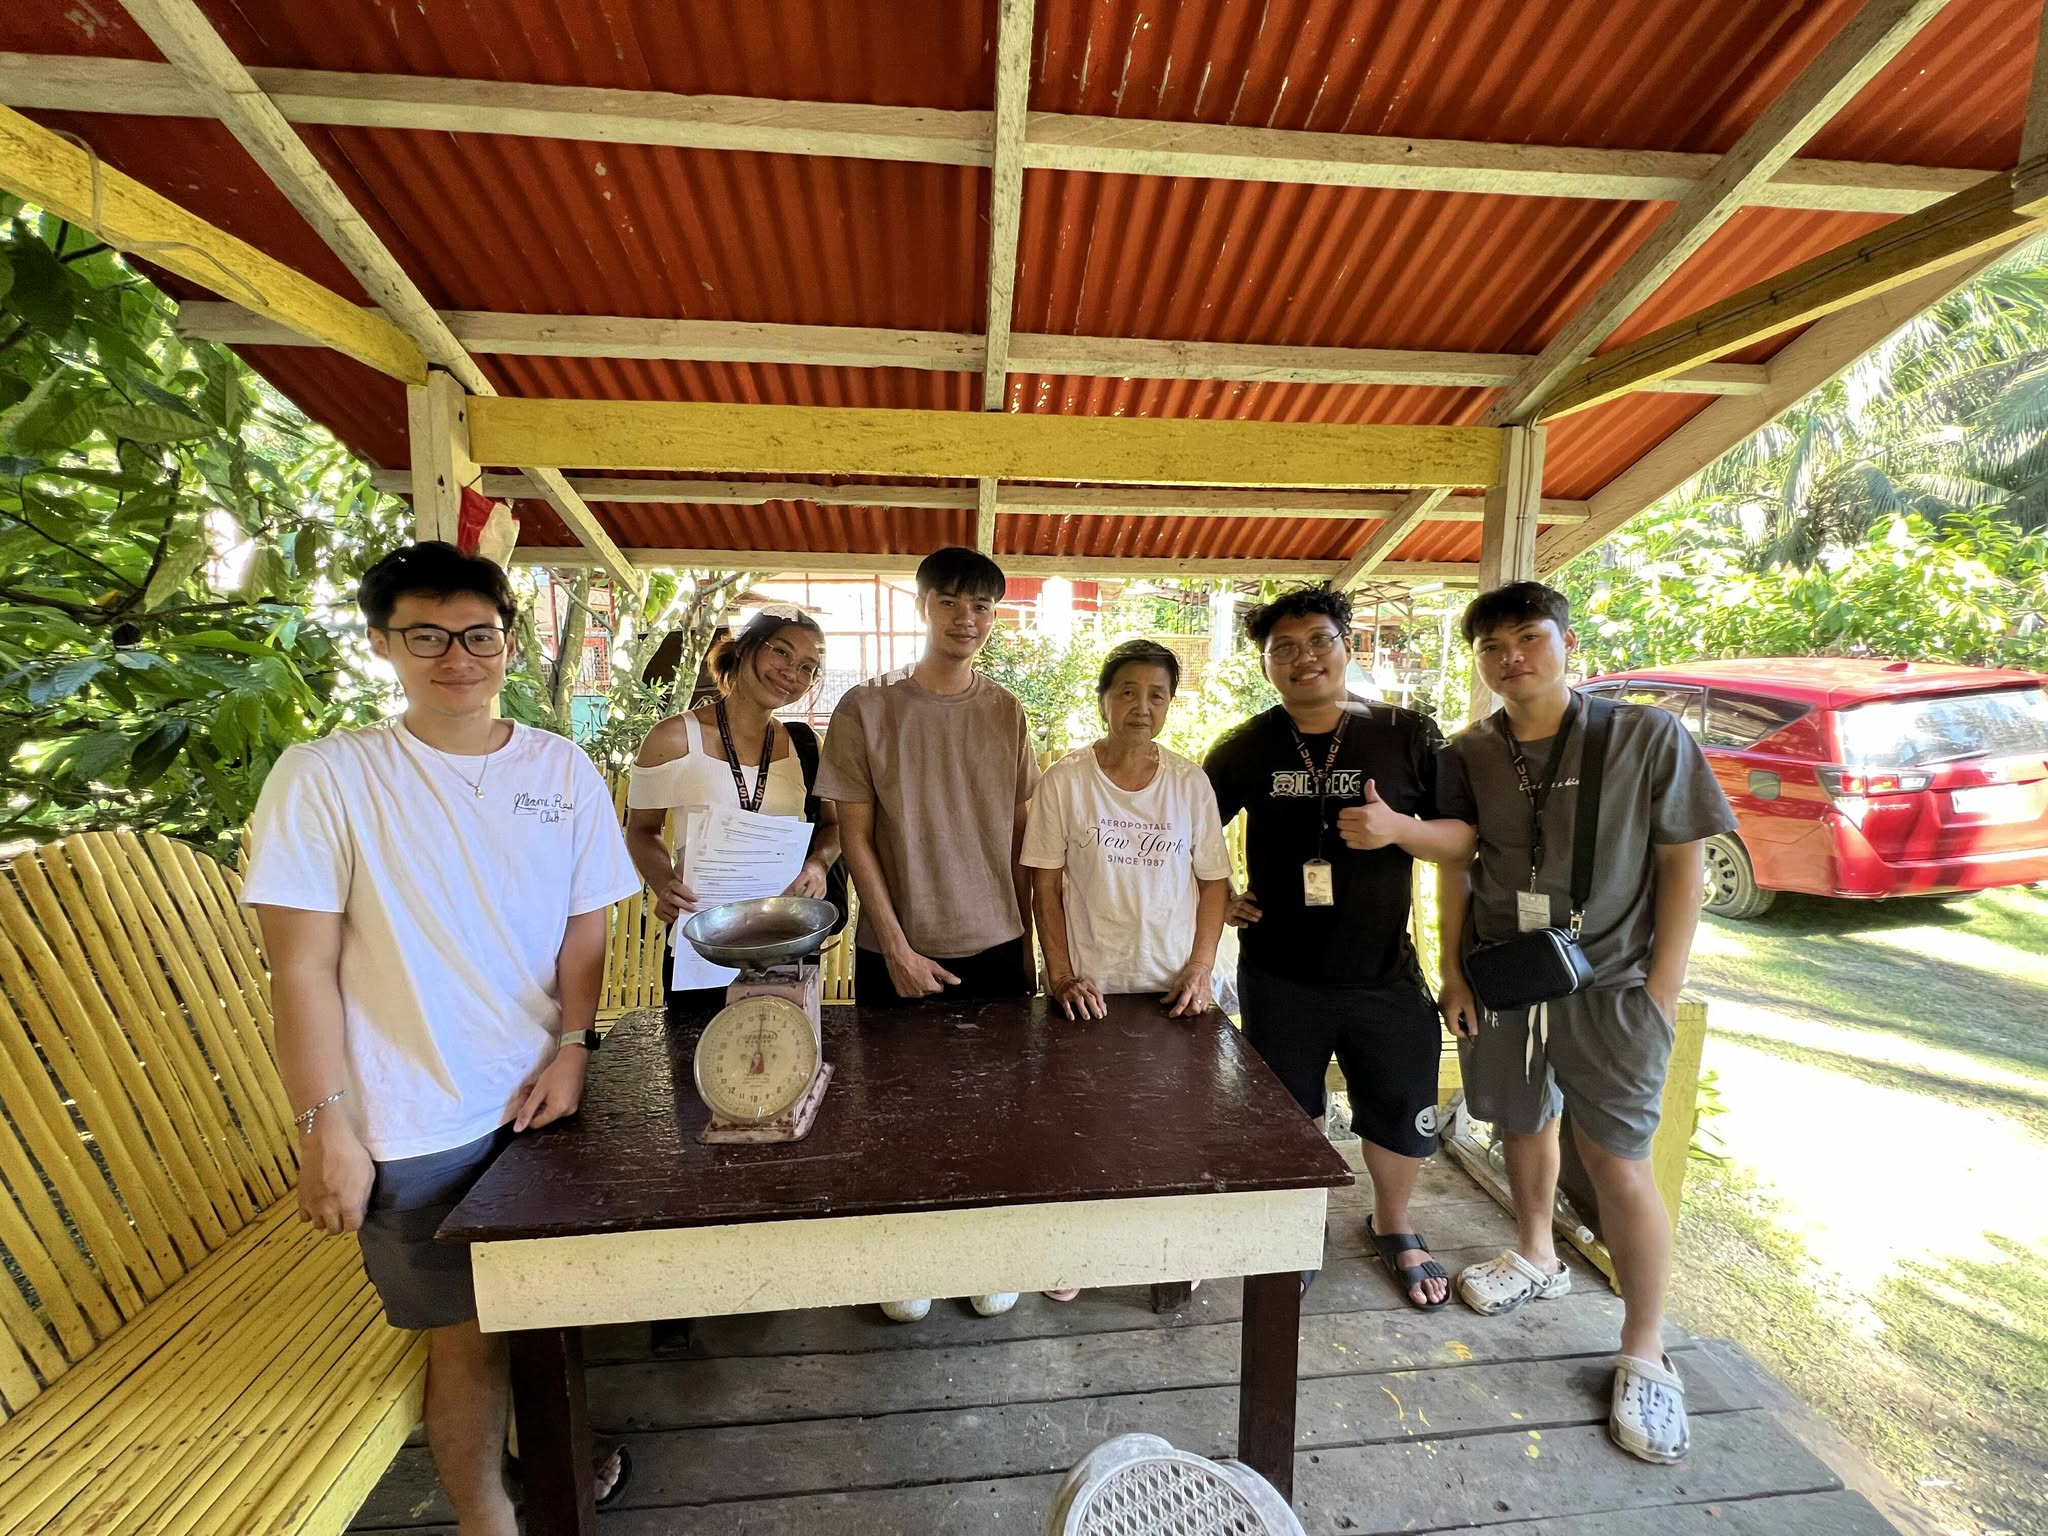
\includegraphics[width=\linewidth]{figures/documentation.jpg}%
		}                                \\ \hline
	\end{longtable}



}
